\documentclass[utf8, a4paper, 11pt, envcountsect]{beamer}

\usepackage[english]{babel}
\usepackage[T1]{fontenc}

\usepackage{amsmath, amsfonts, wrapfig, graphicx}
\usepackage{bm}
\usepackage{mathtools}
\usepackage{stmaryrd}

\usepackage{beamerthemesplit}
\usetheme{CambridgeUS}

\setbeamertemplate{footline}
{\leavevmode%
  \hbox{%
  \begin{beamercolorbox}[wd=\paperwidth,ht=2.25ex,dp=1ex,right]{date in head/foot}%
    \usebeamerfont{date in head/foot}\insertshortdate{}\hspace*{2em}
    \insertframenumber{}-\inserttotalframenumber\hspace*{2ex} \end{beamercolorbox}}%
}

\setbeamertemplate{navigation symbols}{}  % Remove navigation bar
\setbeamertemplate{theorems}[numbered]

\newtheorem{innercustomgeneric}{\customgenericname}
\providecommand{\customgenericname}{}
\newcommand{\newcustomtheorem}[2]{%
  \newenvironment{#1}[1]
  {%
   \renewcommand\customgenericname{#2}%
   \renewcommand\theinnercustomgeneric{##1}%
   \innercustomgeneric}
  {\endinnercustomgeneric}
}

\newcustomtheorem{thm}{Theorem}
\newcustomtheorem{lem}{Lemma}
\newcustomtheorem{cor}{Corollary}
\newcustomtheorem{deftn}{Definition}
\newcustomtheorem{prop}{Proposition}
%\newtheorem{prop}{Proposition}
\DeclareMathOperator*{\argmin}{argmin}
\DeclareMathOperator*{\dist}{dist}
\DeclareMathOperator*{\argmax}{argmax}
\DeclareMathOperator*{\Tr}{Tr}

\title{General ideas on interpolation (B-splines)}
\institute[Uhlmann's lab]{\textbf {V. Uhlmann's lab}}
\author{Yoann Pradat}
\date{\today}
\titlegraphic{
\includegraphics[width=4cm]{EMBL_EBI-logo.png}}

\usepackage[style=alphabetic, backend=bibtex]{biblatex}
\usepackage{csquotes}
\usepackage{filecontents}

\begin{filecontents}{xmpl.bib}
@book{Bo01,
  shorthand = {Bo01},
  author = {Carl de Boor},
  title = {A practical guide to splines},
  year = {2001},
  publisher = {Springer},
  edition = {Revised edition}
}

@article{Bo73,
  shorthand = {Bo73},
  author = {Carl de Boor},
  title = {The quasi-interpolant as a tool in elementary polynomial spline theory},
  year = {1973},
  journal = {J. Approx. Theory},
  pages = {269-276},
}

@book{Ri69,
  shorthand = {Ri69},
  author = {T. Rivlin},
  title = {An introduction to the approximation of functions},
  year = {1969},
  publisher = {Blaisdell}
}

@article{CS66,
  shorthand = {CS66},
  author = {H.B Curry, I.J Schoenberg},
  title = {On Pólya frequency functions IV: the fundamental spline functions and their limits},
  year = {1966},
  journal = {J. Analyse Math.},
  volume = {17},
  pages = {71-107},
}

@article{Bo76,
  shorthand = {Bo76},
  author = {Carl de Boor},
  title = {Splines as linear combinations of B-splines. A survey.},
  year = {1976},
  journal = {J. Approx. Theory},
  volume = {2},
  pages = {1-47},
}

@article{Ma70,
  shorthand = {Ma70},
  author = {M. J. Marsden},
  title = {An identity for spline functions with applications to variation-diminishing spline approximation},
  year = {1970},
  journal = {J. Approx. Theory},
  volume = {3},
  pages = {7-42},
}

@article{Sc46,
  shorthand = {Sc46},
  author = {I.J Schoenberg},
  title = {Contributions to the problem of approximation of equidistant data by analytic functions: part A},
  year = {1946},
  journal = {Quarterly of Applied mathematics},
  volume = {4},
  pages = {45-99},
}

@article{Un99,
  shorthand = {Un99},
  author = {Michael  Unser},
  title = {Splines: A perfect fit for signal and image processing},
  year = {1999},
  journal = {IEEE},
  volume = {16},
  pages = {22-38}
}

\end{filecontents}

\addbibresource{xmpl.bib}

\begin{document}
\frame{\titlepage}

\section[Outline]{}
\frame{\tableofcontents}

\section{Introduction}

%%%%%%%%%%%%%%%
%% FRAME 1
%%%%%%%%%%%%%%%
\frame{\frametitle{Objective}
  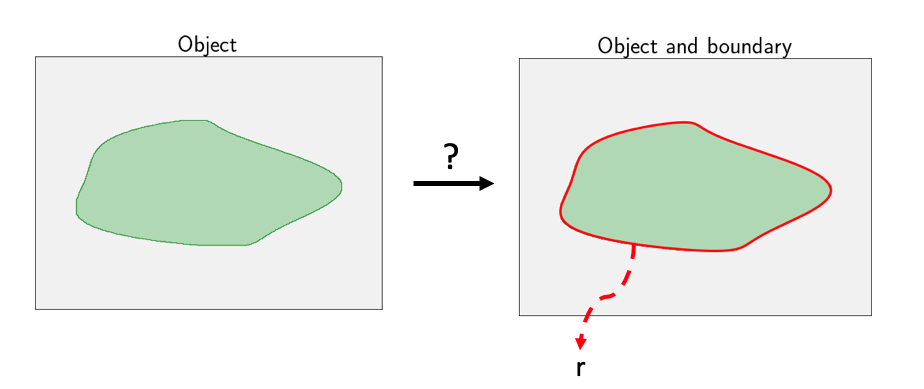
\includegraphics[width=0.9\linewidth]{motivation.png}
  \underline{Objective}: find mathematical model for the \textbf{boundary} 
  \begin{equation}
    {\bf r} = \begin{bmatrix} r_1 \\ \vdots \\ r_d \end{bmatrix}
  \end{equation}
}

%%%%%%%%%%%%%%%
%% FRAME 2
%%%%%%%%%%%%%%%
\frame{\frametitle{Generic model}
  \begin{equation}
    {\bf r}(t) = \begin{bmatrix} r_1 \\ \vdots \\ r_d \end{bmatrix} = \sum_{k \in \mathbb{Z}} \begin{bmatrix} c_1(k) \\ 
    \vdots \\ c_d(k) \end{bmatrix} \phi_k(t)
  \end{equation}
  \underline{Vocab}
  \begin{itemize}
    \item ${(t_k=k)}_{k \in \mathbb{Z}}$ \textbf{knots} locations
    \item ${\bf c}(k) := \begin{bmatrix} c_1(k) \\ \vdots \\ c_d(k) \end{bmatrix}$ are \textbf{control points}
    \item ${(\phi_k)}_{k \in \mathbb{Z}} :=$ set of \textbf{basis functions} or \textbf{generators}
  \end{itemize}
}

\frame{\tableofcontents}

\section{I/ Polynomial interpolation (summary)}

%%%%%%%%%%%%%%%
%% FRAME 3
%%%%%%%%%%%%%%%
\frame{\frametitle{Summary}
  \underline{Not.}
  \begin{itemize}
    \itemsep0em
    \item $f$ agrees with $g$ at $t$ r times if $f^{(j)}(t) = g^{(j)}(t), j=0, \ldots, r-1$
    \item $t_1 \leq \cdots \leq t_n$
    \item $f_n \in \Pi_{<n}$ unique pol\@. order $n$ that agrees with $g$ at ${(t_i)}_{i=1}^n$.
  \end{itemize}
  \begin{deftn}{1}
    $[t_1, \dots, t_n]g$ leading coeff of $f_n$
  \end{deftn}
  \pause%
  \underline{Examples}
  \begin{enumerate}
    \item $[t_1]g = g(t_1)$
    \item $[t_1, t_2]g =\left\{
      \begin{array}{@{}ll@{}}
    \frac{g(t_2)-g(t_1)}{t_2-t_1} & \text{if}\ t_1\neq t_2 \\
    g'(t_1), & \text{otherwise}
  \end{array}\right.$
   \item $[t_1, \ldots, t_{n+1}]g = \frac{[t_2, \ldots, t_{n+1}]g-[t_1, \ldots, t_{n}]g}{t_{n+1}-t_1}$ if $t_1\neq% 
     t_{n+1}$
  \end{enumerate}
}

\frame{\frametitle{Summary}
  \underline{Not.}
  \begin{itemize}
    \itemsep0em
    \item $f$ agrees with $g$ at $t$ r times if $f^{(j)}(t) = g^{(j)}(t), j=0, \ldots, r-1$
    \item $t_1 \leq \cdots \leq t_n$
    \item $f_n \in \Pi_{<n}$ unique pol\@. order $n$ that agrees with $g$ at ${(t_i)}_{i=1}^n$.
  \end{itemize}
  \begin{deftn}{1}
    $[t_1, \dots, t_n]g$ leading coeff of $f_n$
  \end{deftn}
  \begin{thm}{1 (\cite{Bo01}, p7)}
    \setlength{\abovedisplayskip}{-3pt}
    Let $g \in \mathcal{C}^{n}$. Then 
    \begin{equation}
      \forall t, \quad g(t) = f_n(t) + (t-t_1)\dots(t-t_n)[t_1, \dots, t_n, t]g
    \end{equation}
  \end{thm}
  \pause%
  \begin{thm}{2 (Jackson,\cite{Ri69}, p23)}
    \setlength{\abovedisplayskip}{-3pt}
    Let $g \in \mathcal{C}^{r}([a..b]), n > r+1$. Then
    \begin{equation}
      \dist(g, \Pi_{<n}) \leq const_r w(g^{(r)}, \frac{b-a}{2n-1-r}) {\left(\frac{b-a}{n-1}\right)}^r
    \end{equation}
  \end{thm}
  
}

\frame{\tableofcontents}

\section{II/ B-splines and Splines}
\subsection{II/1 Definitions \& Properties}

%%%%%%%%%%%%%%%
%% FRAME 4
%%%%%%%%%%%%%%%
\frame{\frametitle{Formal definition B-splines}
     \underline{Not.}
      \begin{itemize}
        \itemsep0em
        \item $\cdots \leq t_j \leq t_{j+1} \leq \cdots $ finite or infinite
      \end{itemize}
      \pause%
    Two different normalizations
    \begin{deftn}{2 (\cite{Bo01}, p87)}
      The $j^{th}$ (normalized) B-spline of order $k$ is
      \begin{equation}
        B_{j, k, \bm{t}}(t) = (t_{j+k}-t_j)[t_j, \ldots, t_{j+k}]{(.-t)}_+^{k-1}
      \end{equation}
    \end{deftn}
    \pause%
    \begin{deftn}{3 (\cite{CS66})}
      The $j^{th}$ B-spline of order $k$ is given by
      \begin{equation}
        M_{j, k, \bm{t}}(t) = k [t_j, \ldots, t_{j+k}]{(.-t)}_+^{k-1}
      \end{equation}
    \end{deftn}
}

%%%%%%%%%%%%%%%
%% FRAME 5
%%%%%%%%%%%%%%%
\frame{\frametitle{First properties}
  \begin{prop}{1 (\cite{Bo01}, p90--91)}
    \begin{enumerate}
    \item (rec\@. relation)  
      \begin{equation*}
        B_{j, k} = \frac{t-t_j}{t_{j+k-1}-t_j} B_{j, k-1} + \frac{t_{j+k}-t}{t_{j+k}-t_j} B_{j+1, k-1}
      \end{equation*}
    \item (pp function) $B_{j, k, \bm{t}} \in \Pi_{<k, \bm{t}}$
    \item (supp\@. and pos) \begin{itemize}
        \itemsep0em
        \item $B_{j,k} = 0$ outside $[t_j, t_{j+k}]$
        \item $B_{j, k} > 0$ on $(t_j, t_{j+k})$
        \end{itemize}
    \end{enumerate}
  \end{prop}
  \pause%
  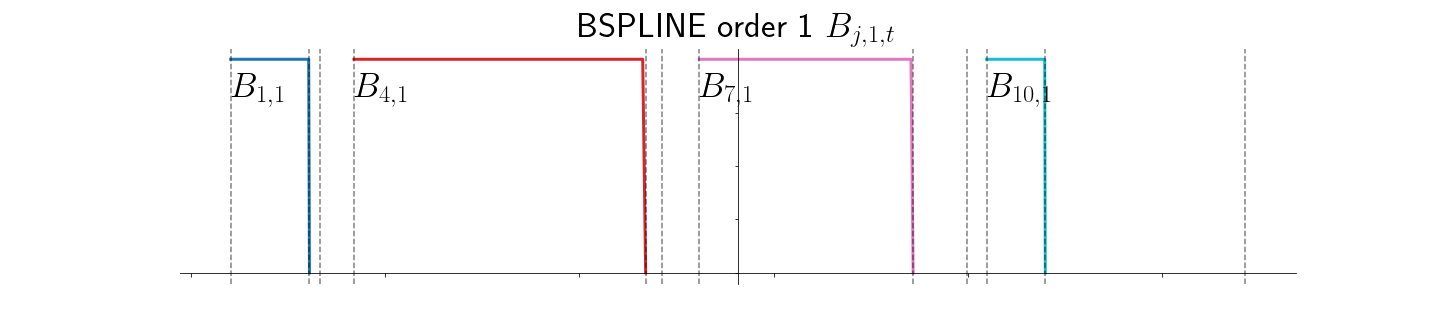
\includegraphics[width=\linewidth]{bspline_order_1.png}
}

\frame{\frametitle{First properties}
  \begin{prop}{1 (\cite{Bo01}, p90--91)}
    \begin{enumerate}
    \item (rec\@. relation)  
      \begin{equation*}
        B_{j, k} = \frac{t-t_j}{t_{j+k-1}-t_j} B_{j, k-1} + \frac{t_{j+k}-t}{t_{j+k}-t_j} B_{j+1, k-1}
      \end{equation*}
    \item (pp function) $B_{j, k, \bm{t}} \in \Pi_{<k, \bm{t}}$
    \item (supp\@. and pos) \begin{itemize}
        \itemsep0em
        \item $B_{j,k} = 0$ outside $[t_j, t_{j+k}]$
        \item $B_{j, k} > 0$ on $(t_j, t_{j+k})$
        \end{itemize}
    \end{enumerate}
  \end{prop}
  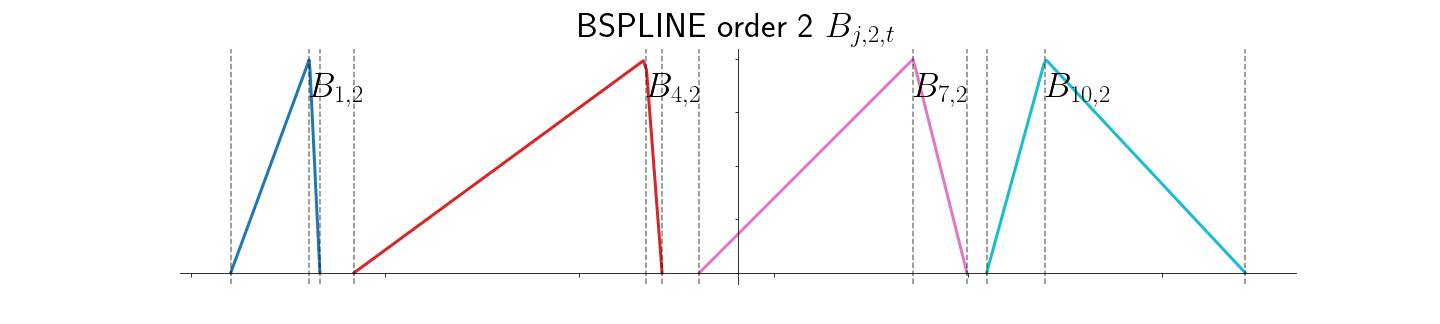
\includegraphics[width=\linewidth]{bspline_order_2.png}
}

\frame{\frametitle{First properties}
  \begin{prop}{1 (\cite{Bo01}, p90--91)}
    \begin{enumerate}
    \item (rec\@. relation)  
      \begin{equation*}
        B_{j, k} = \frac{t-t_j}{t_{j+k-1}-t_j} B_{j, k-1} + \frac{t_{j+k}-t}{t_{j+k}-t_j} B_{j+1, k-1}
      \end{equation*}
    \item (pp function) $B_{j, k, \bm{t}} \in \Pi_{<k, \bm{t}}$
    \item (supp\@. and pos) \begin{itemize}
        \itemsep0em
        \item $B_{j,k} = 0$ outside $[t_j, t_{j+k}]$
        \item $B_{j, k} > 0$ on $(t_j, t_{j+k})$
        \end{itemize}
    \end{enumerate}
  \end{prop}
  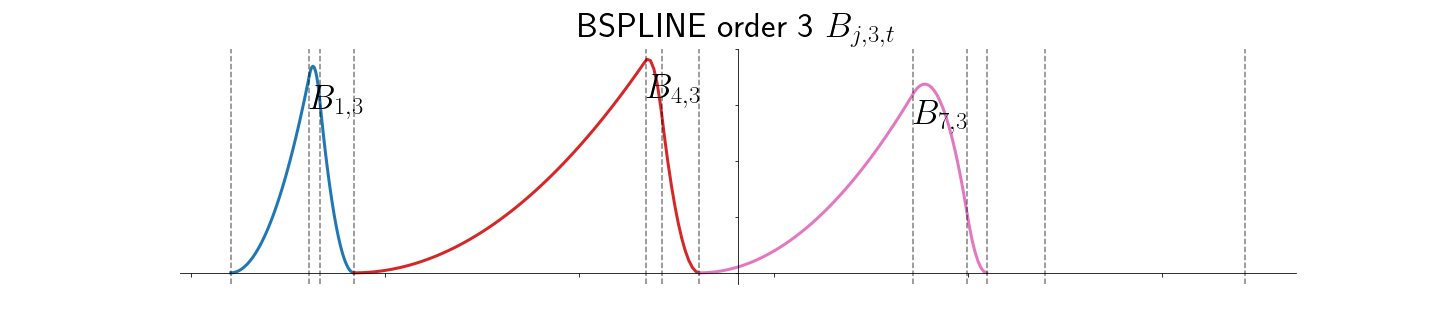
\includegraphics[width=\linewidth]{bspline_order_3.png}
}

\frame{\frametitle{First properties}
  \begin{prop}{1 (\cite{Bo01}, p90--91)}
    \begin{enumerate}
    \item (rec\@. relation)  
      \begin{equation*}
        B_{j, k} = \frac{t-t_j}{t_{j+k-1}-t_j} B_{j, k-1} + \frac{t_{j+k}-t}{t_{j+k}-t_j} B_{j+1, k-1}
      \end{equation*}
    \item (pp function) $B_{j, k, \bm{t}} \in \Pi_{<k, \bm{t}}$
    \item (supp\@. and pos) \begin{itemize}
        \itemsep0em
        \item $B_{j,k} = 0$ outside $[t_j, t_{j+k}]$
        \item $B_{j, k} > 0$ on $(t_j, t_{j+k})$
        \end{itemize}
    \end{enumerate}
  \end{prop}
  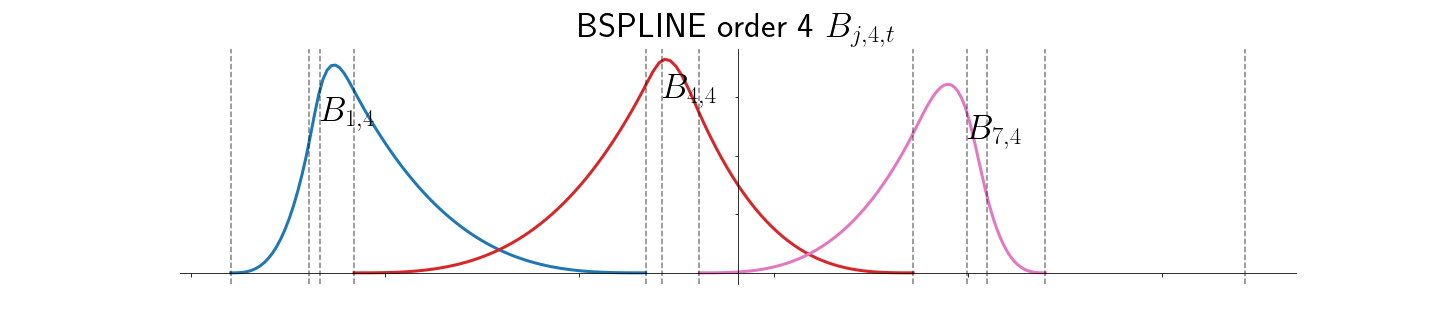
\includegraphics[width=\linewidth]{bspline_order_4.png}
}

\subsection{II/2 The B-spline series}

%%%%%%%%%%%%%%%
%% FRAME 5
%%%%%%%%%%%%%%%
\frame{\frametitle{Why B-splines?}
  \underline{Not.}
  \begin{itemize}
    \itemsep0em
    \item $\bm{t}$ nondecreasing sequence, $\bm{\xi} \subset \bm{t}$ increasing sequence
  \end{itemize}
  \begin{deftn}{4 (\cite{Bo01}, p93)}
    The collection of polynomial splines of order $k$ with knot sequence $\bm{t}$ is
    \begin{equation*}
      \mathcal{S}_{k, {\bm t}} = \{ \sum_{j=-\infty}^{\infty} c(j) B_{j,k, \bm{t}} | \bm{c} \in 
      \mathbb{R}^{\mathbb{Z}}\} \subset \Pi_{<k, \bm{\xi}}
    \end{equation*}
  \end{deftn}
  \pause%
  In (\cite{Bo76}) ``B-splines are truly basic splines: B-splines express the essentially local, but not completely 
  local, character of splines; certain facts about splines take on their most striking form when put into B-spline 
  terms, and many theorems about splines are most easily proved with the aid of B-splines;``
}

%%%%%%%%%%%%%%%
%% FRAME 6
%%%%%%%%%%%%%%%
\frame{\frametitle{Basis for polynomials}
  \begin{enumerate}
    \item (\cite{Ma70},\cite{Bo01} p95) For any $\tau \in \mathbb{R}$,
      \begin{align*}
        {(t-\tau)}^{k-1} &= \sum_{j=-\infty}^{\infty} \psi_{j,k}(\tau) B_{j,k}(t) \\
        \text{where} \quad \psi_{j,k}(\tau) &= (t_j - \tau)\cdots(t_{j+k-1}-\tau)
      \end{align*}
    \item Reproduces $\Pi_{<k}$ i.e $\Pi_{<k} \subset \mathcal{S}_{k,\bm{t}}$
    \item In particular, $\displaystyle \sum_{j=-\infty}^{\infty} B_{j,k} = 1$
  \end{enumerate}
}

\frame{\frametitle{Partition unity}
  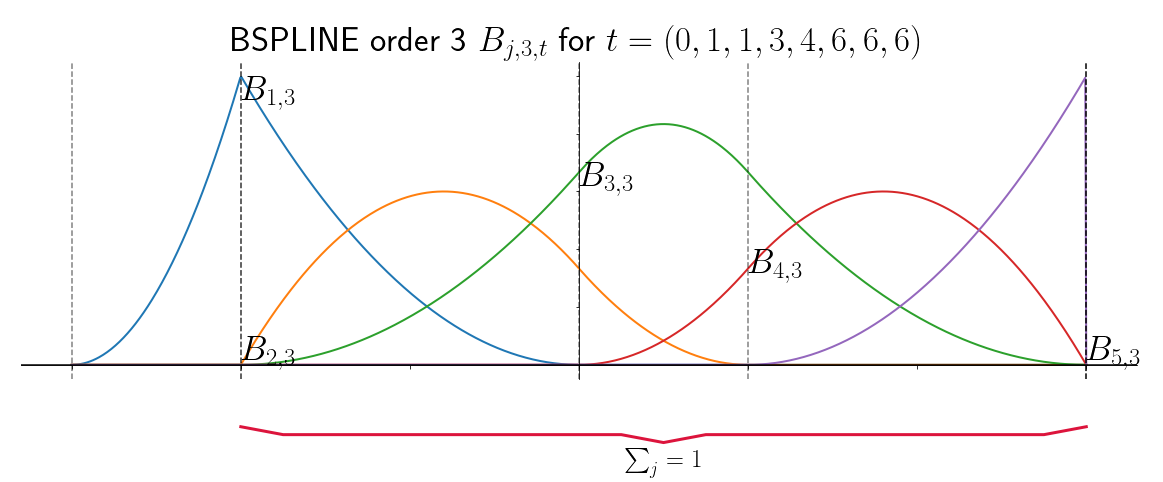
\includegraphics[width=\linewidth]{bspline_mult.png}
}


%%%%%%%%%%%%%%%
%% FRAME 7
%%%%%%%%%%%%%%%
\frame{\frametitle{Basis for $\Pi_{<k, \bm{\xi}, \bm{\nu}}$}
  \underline{Not.}
  \begin{itemize}
    \itemsep0em
    \item $\bm{t}$ nondecreasing sequence with multiplicity $\leq k$.
    \item $\bm{\nu}$ sequence s.t $\nu_j=k - \text{card}\{l| t_l = \xi_j\}$
    \item $\bm{\xi} \subset \bm{t}$ increasing sequence
    \item $\Pi_{<k, \bm{\xi}, \bm{\nu}} = \{f \in \Pi_{<k, \bm{\xi}} \ | \ \text{jump} f^{(s)}_{\xi_j} = 0, s=0,\ldots, 
      \nu_{j}-1\}$
  \end{itemize}
  \pause%
  \begin{thm}{3 (\cite{CS66},\cite{Bo01} p97)}
    ${\{B_{j,k, \bm{t}}\}}_{j=-\infty}^{\infty}$ is a basis for $\Pi_{<k, \bm{\xi}, \bm{\nu}}$ hence $\mathcal{S}_{k,t} 
    = \Pi_{<k, \bm{\xi}, \bm{\nu}}$
  \end{thm}
  \pause%
  \begin{enumerate}
    \item $f \in \mathcal{S}_{k,\bm{t}}$. $f_{|\mathcal{V}(\xi_j)} \in \mathcal{C}^{k-(k-\nu_j)-1}$
    \item $B_{j, k, \bm{\mathbb{Z}}} \in \mathcal{C}^{k-2}$, $B_{j, k, \bm{\mathbb{Z}_r}} \in \mathcal{C}^{k-r-1}$
  \end{enumerate}
}

%%%%%%%%%%%%%%%
%% FRAME 8
%%%%%%%%%%%%%%%
\frame{\frametitle{Knots multiplicity}
  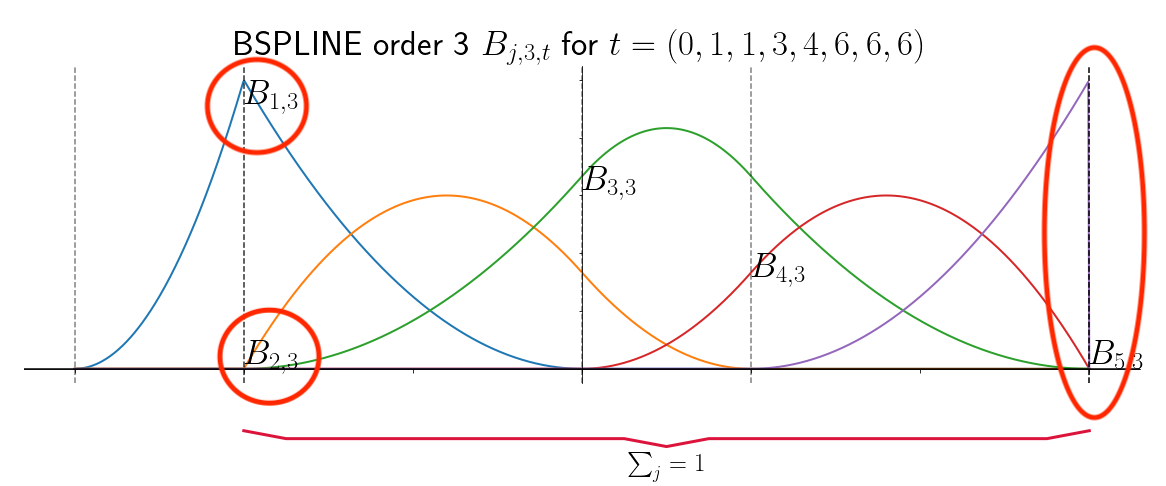
\includegraphics[width=\linewidth]{bspline_mult_emph.png}
}

%%%%%%%%%%%%%%%
%% FRAME 9
%%%%%%%%%%%%%%%
\frame{\frametitle{Good condition for a basis}
  \underline{Riesz-basis $\|\cdot\|_{\infty}$} (\cite{Bo73},\cite{Bo01} p132) \mbox{} \\
  $\exists D_{k} > 0$ independent of $\bm{t}$ such that
  \begin{equation*}
    \forall \bm{c} \in l^{\infty}, \quad D_{k} {\|\bm{c}\|}_{l^{\infty}} \leq {\left\|\sum_{j=-\infty}^{\infty} c_j 
    B_{j,k, \bm{t}}\right\|}_{L^{\infty}} \leq  {\|\bm{c}\|}_{l^{\infty}}
  \end{equation*}
}


\section{III Applications}

\frame{\frametitle{Applications}
  \begin{enumerate}
    \item In practice, choose ${\bm t} = \mathbb{Z}_r$ with $r \geq 1$.
      \begin{itemize}
        \item Landmark paper by Schoenberg~\cite{Sc46}. Splines to interpolate equally spaced data.
            \pause%
        \item~\cite{Un99}
          \begin{equation}
            \beta^0(t) = B_{0,1}(t-\frac{1}{2}), \quad \beta^n(t) = \underbrace{\beta^{0}*\dots*\beta^{0}}_{(n-1) 
            \text{times}}(t)
          \end{equation}
          Signal represented as
          \begin{equation}
            s(t) = \sum_{k=-\infty}^{\infty} c(k) \beta^n(t-k)
          \end{equation}
            Allows for efficient algorithms and Fourier analysis, with $\hat{\beta}^n(w)=  
            {\left(\frac{\sin(\frac{w}{2})}{\frac{w}{2}}\right)}^{n+1}$.
      \end{itemize}
  \end{enumerate}
}

\frame{\frametitle{Applications}
  \begin{enumerate}
    \item In practice, choose ${\bm t} = \mathbb{Z}_r$ with $r \geq 1$.
    \item Critical choice of \textbf{generators} ${\{\phi_j\}}_{j \in \mathbb{Z}}$
      \begin{enumerate}
        \setlength{\abovedisplayskip}{-1pt}
        \setlength{\belowdisplayskip}{-4pt}
        \item Delgado et al. \underline{Snakes with an ellipse-reproducing property}, \emph{IEEE\@}. Vol 21, 2012.
          \begin{equation*}
            r = \sum_{j} \begin{bmatrix} c_1[j] \\ c_2[j] \end{bmatrix} \phi_j \quad \text{with} \ \phi_j = \phi(.-j) 
            \quad \text{with} \quad \phi(t) = \lambda_0 \beta_{\alpha}(t+\frac{3}{2})
          \end{equation*}
          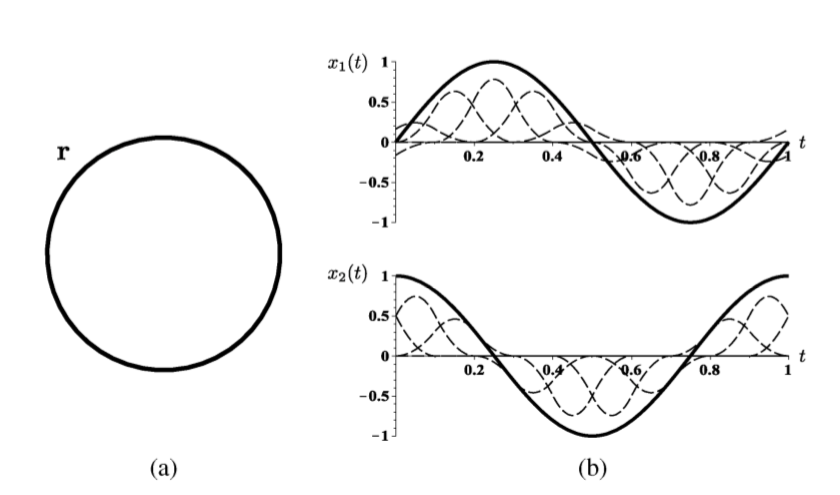
\includegraphics[width=0.8\linewidth]{delgado_2012.png}
      \end{enumerate}
  \end{enumerate}
}

\frame{\frametitle{Applications}
  \begin{enumerate}
    \item In practice, choose ${\bm t} = \mathbb{Z}_r$ with $r \geq 1$.
    \item Critical choice of \textbf{generators} ${\{\phi_j\}}_{j \in \mathbb{Z}}$
      \begin{enumerate}
        \setlength{\abovedisplayskip}{-1pt}
        \setlength{\belowdisplayskip}{-4pt}
        \item Delgado et al. \underline{Snakes with an ellipse-reproducing property}, \emph{IEEE\@}. Vol 21, 2012.
        \item Uhlmann et al. \underline{Hermite snakes with control of tangents}, \emph{IEEE\@}. Vol 25, 2016.
          \begin{equation*}
            r = \sum_{j=-\infty}^{\infty} \begin{bmatrix} c^1_1[j] \\ c^1_2[j] \end{bmatrix} \phi^1_j + \begin{bmatrix} 
          c^2_1[j] \\ c^2_2[j] \end{bmatrix} \phi^2_j \quad \text{with} \ \phi^1_j, \phi^2_j \in \mathcal{S}_{4, 
        \mathbb{Z}_2}            \end{equation*}
          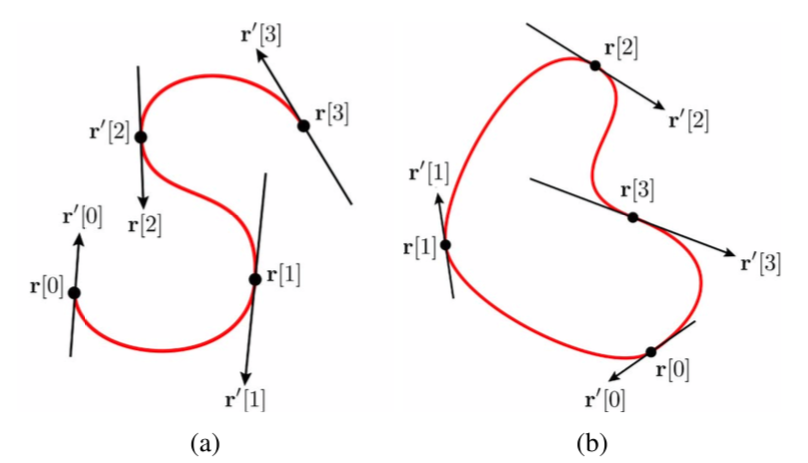
\includegraphics[width=0.65\linewidth]{uhlmann_2016.png}
      \end{enumerate}
  \end{enumerate}
}


\frame{\frametitle{Applications}
  \begin{enumerate}
    \item In practice, choose ${\bm t} = \mathbb{Z}_r$ with $r \geq 1$.
    \item Critical choice of \textbf{generators} ${\{\phi_j\}}_{j \in \mathbb{Z}}$
    \item Things to consider
      \begin{itemize}
        \item Space of reproducible functions
          \begin{equation*}
            V = \text{span}{(\phi_j)} \cap L_2 = \{\sum_{j \in \mathbb{Z}} c[j] \phi_j | c[j] \in \mathbb{R} \} \cap L_2
            \end{equation*}
          \pause%
          \item Desired properties in CAGD
            \begin{enumerate}
              \item Affine invariance i.e $s \in V \implies As + b \in V$. True if $\sum_j \phi_j = 1$
              \item Unicity and stability. True if $(\phi_j)$ is a Riesz-basis in $L_2$ i.e $\exists 0 < m, M$
                \begin{equation*}
                  m {\|c\|}_{l_2}^2 \leq {\left\|\sum_{j}  c[j] \phi_j \right\|}_{L_2}^2 \leq  M{\|c\|}_{l_2}^2
              \end{equation*}
            \end{enumerate}
         \pause%
       \item Reproducible functions
         \begin{enumerate}
           \item Polynomial, exponential polynomials
           \item Smoothness
         \end{enumerate}
       \pause%
       \item Approximation power as number of control points increases
    \end{itemize}
  \end{enumerate}
}

\begin{frame}[allowframebreaks]
  \frametitle{References}
  \printbibliography%
 \end{frame}


\end{document}
